\documentclass[conference]{IEEEtran}
\IEEEoverridecommandlockouts
\usepackage{cite}
\usepackage{amsmath,amssymb,amsfonts}
\usepackage{graphicx}
\usepackage{textcomp}
\usepackage{xcolor}
\usepackage{booktabs}
\usepackage{multirow}
\usepackage{tikz}
\usetikzlibrary{arrows.meta,positioning,fit,backgrounds}
\usepackage[hidelinks]{hyperref}

\newcommand{\nTurns}{30{,}015}
\newcommand{\nSessions}{6{,}828}
\newcommand{\nUsers}{2{,}501}
\newcommand{\nCandTurns}{12{,}124}
\newcommand{\nLabeledTurns}{10{,}776}
\newcommand{\labelCoverage}{88.9\%}
\newcommand{\nPickPairs}{199}
\newcommand{\judgeAgreeRange}{85--88\%}
\newcommand{\nNearPairs}{7{,}360}
\newcommand{\nearWrongAll}{56.3\%}
\newcommand{\nearWrongDep}{75.7\%}
\newcommand{\nearWrongSelf}{37.1\%}
\newcommand{\nearWrongCandDep}{73.2\%}
\newcommand{\nearWrongCandSelf}{42.2\%}
\newcommand{\resultSentence}{On the held-out period, behavior-aware admission serves 4.49\% of all requests at a 10\% wrong-reuse level against 0.02\% for a fixed similarity threshold and 0.80\% for per-intent thresholds, significant against the fixed threshold at both pre-registered levels, and mined patterns remove wrong reuse on corrections; against a learned per-turn verifier the aggregate gain is not significant.}
\newcommand{\resultParagraph}{Table~\ref{tab:main} and Fig.~\ref{fig:curves} report the single confirmation run on frozen code. Every learned policy serves far more requests than similarity thresholds at the same wrong-reuse level. At $\alpha=10\%$ the pattern-aware policy P4 serves 4.49\% of all requests, against 0.02\% for the fixed threshold and 0.80\% for per-intent thresholds; its gain over the fixed threshold is significant at both levels after Holm correction (+1.10 and +4.47 points). Against the per-turn verifier P3 and the context-embedding policy P5, P4 is statistically indistinguishable (-0.13 and +0.62 points at 10\%, intervals including zero), so the pre-registered criterion, which required P4 to beat every comparator, is not met. Most of the behavioral signal that drives volume is therefore already carried by per-turn dialogue acts, which P3 uses; the mined patterns change \emph{which} requests are served rather than how many.}
\newcommand{\controlsParagraph}{Neither placebo (each session's history shuffled, or borrowed from another session) nor any ablation differs from P3 at either level (Table~\ref{tab:controls}), consistent with the main result. The mechanism analysis, fixed before the run, shows where the patterns act: at the operating point with at most 10\% wrong reuse, P4 removes wrong reuse on corrections (from 66.7\% to 0.0\%), lowers it on follow-ups (15.4\% to 13.3\%) and on later turns of a session (11.4\% to 10.2\%), at a small cost in hits. The advantage over the fixed threshold survives a stricter similarity floor of 0.80 (+1.59 and +4.34 points, both significant). A positive control with injected behavior-dependent duplicates confirms that the pipeline detects pattern effects when they exist: the pattern-aware verifier serves 24.0\% at 10\% wrong reuse against 5.7\% for the per-query verifier.}
\newcommand{\routingParagraph}{On 1{,}377 multi-turn conversations in which human voters compared a strong and a weak model~\cite{lmsys2024arena55k}, the weak model was at least as good in 45.8\% of cases. With the strong model limited to 30\% of requests, routers reach a quality of 61.1\% (per-query), 62.7\% (context) and 61.9\% (patterns), against 62.1\% for random routing at the same budget; at 50\% the values are 73.3\%, 73.1\% and 72.3\% against 72.9\% at random. Conversation-level votes on this sample carry little routing signal for any router. The pattern router's gain over the per-query router is +0.73 and -1.02 points (not significant after Holm correction). Fig.~\ref{fig:routing} shows the full trade-off.}
\newcommand{\trajectoryParagraph}{Of 710 satisfied multi-turn sessions in the confirmation period, every one had an earlier stored trajectory with the same opening intent; we judged the 83 closest matches. Only 4.8\% of fast-tracks would have given the user what they eventually needed, and even among sessions whose opening request was identical to the stored one the false fast-track rate was 100.0\%. Turns saved stay near zero (0.025 per session) against an oracle of 4.70. Conversations that open the same way end in different places, which is the behavioral effect of Section~\ref{sec:finding} at the level of whole sessions: trajectories have to be matched on behavior as it unfolds, not on the opening request. This analysis is exploratory and its satisfaction proxy awaits human validation.}
\newcommand{\serviceParagraph}{The admission service decides in 43.4 ms at the median and 79.0 ms at the 95th percentile on a laptop CPU with 3{,}000 cached entries, including embedding the request; this is small next to the seconds a provider call takes.}
\newcommand{\conclusionSentence}{On a held-out period it served 4.49\% of requests at a 10\% wrong-reuse level, about 240 times a fixed-threshold cache, and removed wrong reuse on corrections; whether mined patterns also add volume beyond per-turn dialogue acts remains open at our scale.}


\begin{document}

\title{Pattern-Mining-Driven Cache Admission and Routing for Multi-Provider LLM Gateways}

\author{
\IEEEauthorblockN{1\textsuperscript{st} Arnav Gupta}
\IEEEauthorblockA{\textit{School of Computer Science and Engineering} \\
\textit{VIT-AP University}\\
Amaravati, India \\
email}
\and
\IEEEauthorblockN{2\textsuperscript{nd} Author Name}
\IEEEauthorblockA{\textit{School of Computer Science and Engineering} \\
\textit{VIT-AP University}\\
Amaravati, India \\
email}
\and
\IEEEauthorblockN{3\textsuperscript{rd} Author Name}
\IEEEauthorblockA{\textit{School of Computer Science and Engineering} \\
\textit{VIT-AP University}\\
Amaravati, India \\
email}
\and
\IEEEauthorblockN{4\textsuperscript{th} Author Name}
\IEEEauthorblockA{\textit{School of Computer Science and Engineering} \\
\textit{VIT-AP University}\\
Amaravati, India \\
email}
}

\maketitle

\begin{abstract}
Semantic caches in large language model (LLM) gateways decide whether to reuse a stored answer by comparing one incoming request with earlier requests, one query at a time. We show that this view misses what actually determines whether reuse is safe in conversational traffic: the behavioral role of the request and of the cached entry. On \nTurns{} turns of real multi-turn chatbot traffic, with every candidate reuse judged against the answer the user actually received, a similarity cache returns an unacceptable answer for \nearWrongAll{} of near-duplicate requests. At the same similarity, follow-ups, continuations and corrections are wrong \nearWrongDep{} of the time against \nearWrongSelf{} for self-contained requests. We introduce behavior-aware admission: dialogue acts and intents are mined into frequent and sequential patterns per session and per user, every request and cache entry is placed in a mined behavioral state, and class association rules over pairs of states give a reuse-safety prior that enters an expected-benefit admission rule. We evaluate with a stateful gateway replay in which every policy keeps its own cache, a reference-based LLM judge, pre-registered criteria and a single confirmation run on a held-out later period. \resultSentence{} We release the full pipeline, a live admission service and the evaluation protocol.
\end{abstract}

\begin{IEEEkeywords}
semantic caching, LLM gateway, sequential pattern mining, association rules, dialogue acts, model routing
\end{IEEEkeywords}

\section{Introduction}
Organizations increasingly place a gateway between their applications and several LLM providers. The gateway authenticates traffic, enforces budgets, routes each request to a model and, increasingly, answers repeated requests from a cache. Semantic caching extends exact-match caching by reusing an answer whenever a new request is close enough to a stored one in embedding space~\cite{bang2023gptcache}. Follow-up work learns better similarity models~\cite{gill2025meancache}, adapts thresholds per embedding region~\cite{schroeder2025vectorq} or per query category~\cite{wang2025category}, and adds conversational context to the match~\cite{yan2025contextcache}.

All of these systems treat admission as a property of one request, possibly with its recent context, measured against one stored request. Real gateway traffic is not like that. Users iterate: they paste material and ask for a summary, then for key points, then for a shorter version; they say ``continue'', ``try again'' or ``that is wrong''. Two requests can be textually identical and still need different answers, because one is a fresh question and the other refers to an answer the user has just seen. Conversely, a cached answer that was itself produced in the middle of a refinement loop is a poor answer to a fresh question, however similar the two requests look. The decision depends on behavior, and behavior has structure that recurs across sessions and users.

This paper asks whether that structure can be mined and used. Our hypothesis is that behavioral patterns mined from gateway traffic improve cache admission (and model routing) compared with fixed-threshold and per-query similarity policies. We make the following contributions.

\begin{itemize}
\item \textbf{A quantified failure mode of similarity caching.} On \nTurns{} real chatbot turns, judged against the answer each user actually received, we show that reuse safety is governed by dialogue behavior: at near-duplicate similarity, context-dependent requests are wrong roughly twice as often as self-contained ones, on both the request and the cache-entry side (Section~\ref{sec:finding}).
\item \textbf{Behavior-aware admission.} We mine frequent itemsets (FP-Growth~\cite{han2000fpgrowth}) and sequential patterns (PrefixSpan~\cite{pei2001prefixspan}) over dialogue acts and intents per session and per user, re-mined daily from past traffic only. We define the behavioral state of a request and of a cache entry, and learn class association rules~\cite{liu1998cba} over state pairs that act as a reuse-safety prior inside an expected-benefit decision rule (Section~\ref{sec:method}). To our knowledge this is the first semantic cache that conditions admission on mined behavioral patterns of both sides of a reuse.
\item \textbf{A rigorous evaluation protocol for cache admission.} A stateful replay keeps a separate cache per policy, labels come from a reference-based judge validated against human raters, metrics are read at matched wrong-reuse levels, and the claims, comparators and pass rule are pre-registered and tested once on a later, held-out period (Section~\ref{sec:setup}).
\item \textbf{Extensions to routing and trajectory caching.} The same mined patterns feed a strong/weak model router evaluated on human preference votes, and an exploratory trajectory cache that fast-tracks conversations to the answer that satisfied similar users (Sections~\ref{sec:routing} and~\ref{sec:trajectory}).
\end{itemize}

\section{Related Work}
\label{sec:related}
\textbf{Semantic caching.} GPTCache~\cite{bang2023gptcache} popularized embedding-based reuse with a global similarity threshold. MeanCache~\cite{gill2025meancache} keeps per-user caches and learns the similarity model with federated learning. VectorQ~\cite{schroeder2025vectorq} replaces the global threshold with learned per-embedding threshold regions, and category-aware caching~\cite{wang2025category} varies thresholds, time-to-live and quotas by query category. ContextCache~\cite{yan2025contextcache} adds the dialogue history to the match through attention over earlier turns. Table~\ref{tab:positioning} positions our work: earlier systems decide from the similarity of the current request (with or without its context); ours additionally conditions on mined, recurring behavioral patterns of both the request and the cached entry.

\textbf{Model routing.} FrugalGPT~\cite{chen2024frugalgpt} cascades models to cut cost, and RouteLLM~\cite{ong2025routellm} learns strong/weak routers from human preference data collected on Chatbot Arena~\cite{chiang2024arena}. These routers score one prompt at a time; we add mined session patterns as router features.

\textbf{Pattern mining and dialogue quality.} Frequent-pattern and sequential-pattern mining~\cite{han2000fpgrowth,pei2001prefixspan} and associative classification~\cite{liu1998cba} are classical tools that, to our knowledge, have not been used for LLM cache admission. User-satisfaction estimation over multi-turn dialogue~\cite{bodigutla2020satisfaction} motivates our satisfaction proxy for trajectory caching. LLM judges~\cite{zheng2023judge} are now a common way to score open-ended responses; we use one with a reference answer and validate it against human raters.

\begin{table}[t]
\caption{Positioning against prior semantic caches and routers}
\label{tab:positioning}
\centering
\footnotesize
\begin{tabular}{@{}lccc@{}}
\toprule
System & Decision signal & Uses context & Mined behavior \\
\midrule
GPTCache~\cite{bang2023gptcache} & global threshold & no & no \\
MeanCache~\cite{gill2025meancache} & learned similarity & no & no \\
VectorQ~\cite{schroeder2025vectorq} & per-region threshold & no & no \\
Category-aware~\cite{wang2025category} & per-category policy & no & no \\
ContextCache~\cite{yan2025contextcache} & attention over history & yes & no \\
RouteLLM~\cite{ong2025routellm} (routing) & per-prompt router & no & no \\
\textbf{This work} & \textbf{rule prior + verifier} & \textbf{yes} & \textbf{yes} \\
\bottomrule
\end{tabular}
\end{table}

\section{Behavior-Aware Admission}
\label{sec:method}

\begin{figure*}[t]
\centering
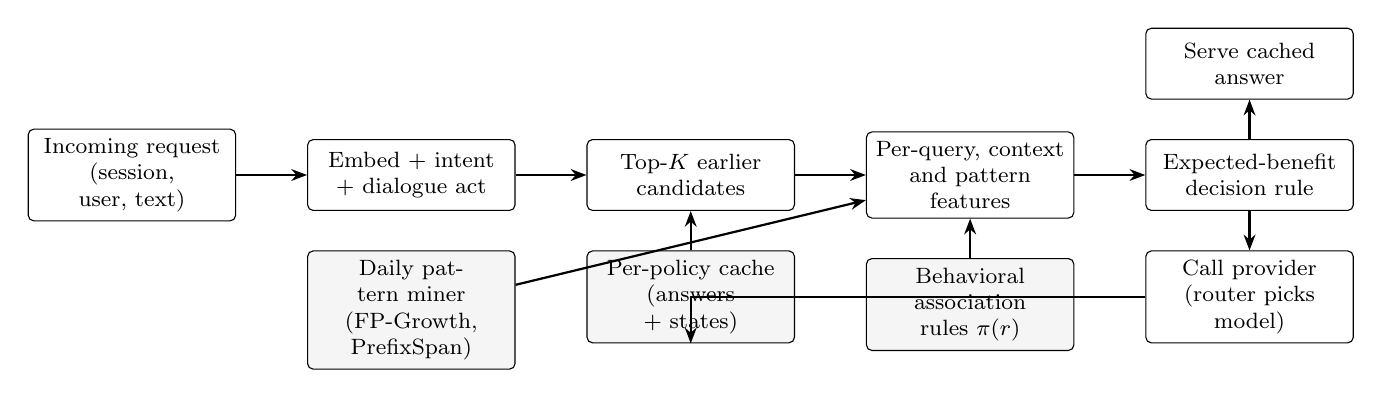
\begin{tikzpicture}[
  node distance=5mm and 9mm,
  box/.style={draw, rounded corners=2pt, align=center, font=\footnotesize, minimum height=9mm, text width=24mm, fill=white},
  store/.style={box, fill=black!4},
  arr/.style={-{Stealth[length=2mm]}, thick}]
\node[box] (req) {Incoming request\\(session, user, text)};
\node[box, right=of req] (emb) {Embed + intent\\+ dialogue act};
\node[box, right=of emb] (cand) {Top-$K$ earlier\\candidates};
\node[box, right=of cand] (feat) {Per-query, context\\and pattern features};
\node[box, right=of feat] (dec) {Expected-benefit\\decision rule};
\node[store, below=of emb] (miner) {Daily pattern miner\\(FP-Growth, PrefixSpan)};
\node[store, below=of cand] (cache) {Per-policy cache\\(answers + states)};
\node[store, below=of feat] (rules) {Behavioral association\\rules $\pi(r)$};
\node[box, above=of dec] (serve) {Serve cached answer};
\node[box, below=of dec] (fresh) {Call provider\\(router picks model)};
\draw[arr] (req) -- (emb);
\draw[arr] (emb) -- (cand);
\draw[arr] (cand) -- (feat);
\draw[arr] (feat) -- (dec);
\draw[arr] (dec) -- (serve);
\draw[arr] (dec) -- (fresh);
\draw[arr] (miner) -- (feat);
\draw[arr] (cache) -- (cand);
\draw[arr] (rules) -- (feat);
\draw[arr] (fresh.west) -| (cache.south);
\end{tikzpicture}
\caption{Gateway with behavior-aware admission. Patterns are re-mined daily from past traffic; association rules are learned from labeled past reuses; every policy keeps its own cache, so an answer served from cache never becomes a cache entry.}
\label{fig:arch}
\end{figure*}

\subsection{Problem setting}
A gateway receives turns $t=1,2,\dots$ in time order. Turn $t$ has a session $s_t$, a user $u_t$, a request $x_t$ and, once answered, a response $y_t$. When $x_t$ arrives, the cache holds earlier answered turns. Let $\mathcal{C}_t$ be the $K$ cached turns most similar to $x_t$ under cosine similarity $\mathrm{sim}(\cdot,\cdot)$ of sentence embeddings~\cite{reimers2019sbert,wang2020minilm}, restricted to similarity at least $\rho$. Admission chooses either one candidate $c\in\mathcal{C}_t$, whose answer $y_c$ is returned, or a fresh provider call. A reuse is \emph{acceptable} when $y_c$ serves $x_t$ as well as the answer the user actually received.

\subsection{Behavioral tokens}
Each turn receives an intent $\iota_t$ (one of $k$ clusters of request embeddings, fit on the training period) and a dialogue act $a_t \in \{$new request, follow-up, continuation, correction, new ask on the same material$\}$. Intents capture \emph{what} is asked; acts capture \emph{how the turn relates to the conversation}, which is what the failure mode above depends on.

\subsection{Pattern mining}
For an entity $e$ (a session, or a user across sessions) let $\mathrm{seq}(e)$ be its token sequence. The support of a pattern $p$ over a set of entities $E$ and the confidence of a sequential rule are
\begin{align}
\mathrm{supp}(p) &= \frac{|\{e\in E : p \sqsubseteq \mathrm{seq}(e)\}|}{|E|}, \label{eq:supp}\\
\mathrm{conf}(a_{1:k} \Rightarrow b) &= \frac{\mathrm{supp}(a_1 \dots a_k\, b)}{\mathrm{supp}(a_1 \dots a_k)}, \label{eq:conf}
\end{align}
where $\sqsubseteq$ denotes subsequence containment. Itemsets over $(\iota,a)$ tokens are mined with FP-Growth and sequences of length up to three with PrefixSpan. Mining is repeated every day using only traffic that arrived before that day, so no feature of a turn depends on later traffic.

\subsection{Behavioral states and association rules}
The behavioral state of a turn with act history $h=(a_1,\dots,a_m)$ is the longest suffix of length at most two that the miner found frequent,
\begin{equation}
\sigma(h) = \begin{cases} \text{start} & m=0,\\ \arg\max_{\ell\le 2}\{h_{m-\ell+1:m} : h_{m-\ell+1:m}\in\mathcal{F}\} & \text{if one exists},\\ \text{rare} & \text{otherwise}, \end{cases}
\end{equation}
where $\mathcal{F}$ is the set of frequent act sequences. For a request $x_t$ and a candidate $c$ we form the rule key $r=(\sigma_t, a_t, \sigma_c, a_c)$, combining the state and act of both sides of the reuse. From labeled past reuses we estimate a smoothed class association rule~\cite{liu1998cba}
\begin{equation}
\pi(r) = \frac{\sum_{i\in r} y_i + m\,\bar y}{n_r + m}, \label{eq:rule}
\end{equation}
where $y_i\in\{0,1\}$ marks acceptable reuse, $n_r$ is the number of labeled pairs under rule $r$, $\bar y$ is the overall acceptance rate and $m$ a pseudo-count. Training rows receive out-of-fold estimates so that no row's prior uses its own label.

\subsection{Expected-benefit admission}
For every candidate $c\in\mathcal{C}_t$ a gradient-boosted verifier~\cite{ke2017lightgbm} estimates $f(z_c)=\Pr(\text{acceptable}\mid z_c)$ from a feature vector $z_c$ that contains the similarity profile (including the softmax share $\exp(\mathrm{sim}_c/\tau)/\sum_{j}\exp(\mathrm{sim}_j/\tau)$), intents, acts, lengths and time gap; in the pattern-aware policy it also contains the mined pattern features and $\pi(r)$. The probability that the answer is still valid decays with age $\Delta_c$ (half-life $T$), and admission serves the candidate with the highest expected benefit when it is positive enough:
\begin{align}
q_c &= f(z_c)\cdot 2^{-\Delta_c/T}, \\
B_c &= U\,q_c - L\,(1-q_c), \label{eq:benefit}\\
\text{serve } c^\star &= \arg\max_{c} B_c \quad \text{iff} \quad B_{c^\star}\ge\theta, \label{eq:decision}
\end{align}
where $U$ is the value of a correct reuse and $L$ the cost of a wrong one. Sweeping $\theta$ traces the trade-off between serving more requests and serving more wrong answers.

\section{Experimental Setup}
\label{sec:setup}
\subsection{Data}
We replay \nTurns{} English multi-turn turns (\nSessions{} sessions, \nUsers{} hashed users) from WildChat~\cite{zhao2024wildchat}, keeping each request together with the answer the user received. Sessions are assigned by the time of their first turn to a training period (60\%), a development period (20\%) and a later confirmation period (20\%). Embeddings use all-MiniLM-L6-v2~\cite{reimers2019sbert,wang2020minilm} with exact inner-product search~\cite{johnson2021faiss}. Every turn's dialogue act is tagged by an LLM. Candidates are the top three earlier turns with similarity at least 0.70; \nCandTurns{} turns have at least one.

\subsection{Ground truth}
A judge model sees the new request, the answer the user actually received (the reference), and each candidate's request and answer, and decides for each candidate whether returning its answer would have been acceptable. Three judge models labeled the same \nPickPairs{} pairs and agreed on \judgeAgreeRange{} of them; the mid-sized model was chosen as the judge for cost. These pairs also form the human gold set (two independent raters per pair). Turns were labeled in a random order that is stratified by period and similarity band, so any labeled prefix is a stratified sample; \nLabeledTurns{} turns (\labelCoverage{}) were labeled, and all metrics are reweighted to the stratum populations.

\subsection{Policies}
We compare six admission policies: \textbf{P1} a fixed cosine threshold; \textbf{P2} per-intent calibrated thresholds; \textbf{P3} the learned per-query verifier; \textbf{P5} P3 plus context-embedding similarities in the style of ContextCache~\cite{yan2025contextcache}; \textbf{P4} P3 plus mined pattern features and the rule prior $\pi$; and \textbf{P4+} P5 plus the same pattern features. P4 versus P3 isolates the contribution of mined behavior; P4 versus P5 tests it against raw context.

\subsection{Replay and metrics}
Each policy replays the entire stream with its own cache: an answer served from cache never enters it, so earlier decisions change later options. With population weights $w_t=N_{p,b}/n_{p,b}$ for a labeled turn in period $p$ and similarity band $b$, and $N$ turns in the evaluation period, the hit rate and wrong-reuse rate at threshold $\theta$ are
\begin{align}
\mathrm{HR}(\theta) &= \frac{1}{N}\sum_t w_t\,\mathbb{1}[\text{served}_t(\theta)], \\
\mathrm{WR}(\theta) &= \frac{\sum_t w_t\,\mathbb{1}[\text{served}_t(\theta)\wedge\neg\text{acc}_t]}{\sum_t w_t\,\mathbb{1}[\text{served}_t(\theta)]},
\end{align}
and the primary readout is the hit rate at a matched wrong-reuse level $\alpha\in\{5\%,10\%\}$:
\begin{equation}
\mathrm{HR}@\alpha = \max_\theta\,\{\mathrm{HR}(\theta) : \mathrm{WR}(\theta)\le\alpha\}. \label{eq:hra}
\end{equation}
Uncertainty comes from 1000 session-level bootstrap resamples~\cite{efron1993bootstrap} of the paired difference between P4 and each comparator, with Holm correction~\cite{holm1979} across the two levels. Before the confirmation data were evaluated we fixed the pass rule: P4 must beat P1, P2, P3 and P5 at both levels with corrected intervals excluding zero. All design changes were logged with dates before a single run on frozen code.

\section{Results}
\label{sec:results}

\subsection{Behavior governs reuse safety}
\label{sec:finding}
Fig.~\ref{fig:finding} breaks the judged wrong-reuse rate down by similarity band and by the dialogue act of the new request. Similarity matters, but at every band the act matters more than the remaining similarity differences: among near-duplicates ($\mathrm{sim}\ge 0.97$, \nNearPairs{} pairs) the wrong-reuse rate is \nearWrongSelf{} for self-contained requests and \nearWrongDep{} for context-dependent ones. The same split holds on the cache side: answers produced by context-dependent turns are wrong for a new request \nearWrongCandDep{} of the time against \nearWrongCandSelf{} for answers to self-contained turns. A per-query similarity cache cannot see either effect. Table~\ref{tab:rules} lists mined association rules at the extremes.

\begin{figure}[t]
\centering
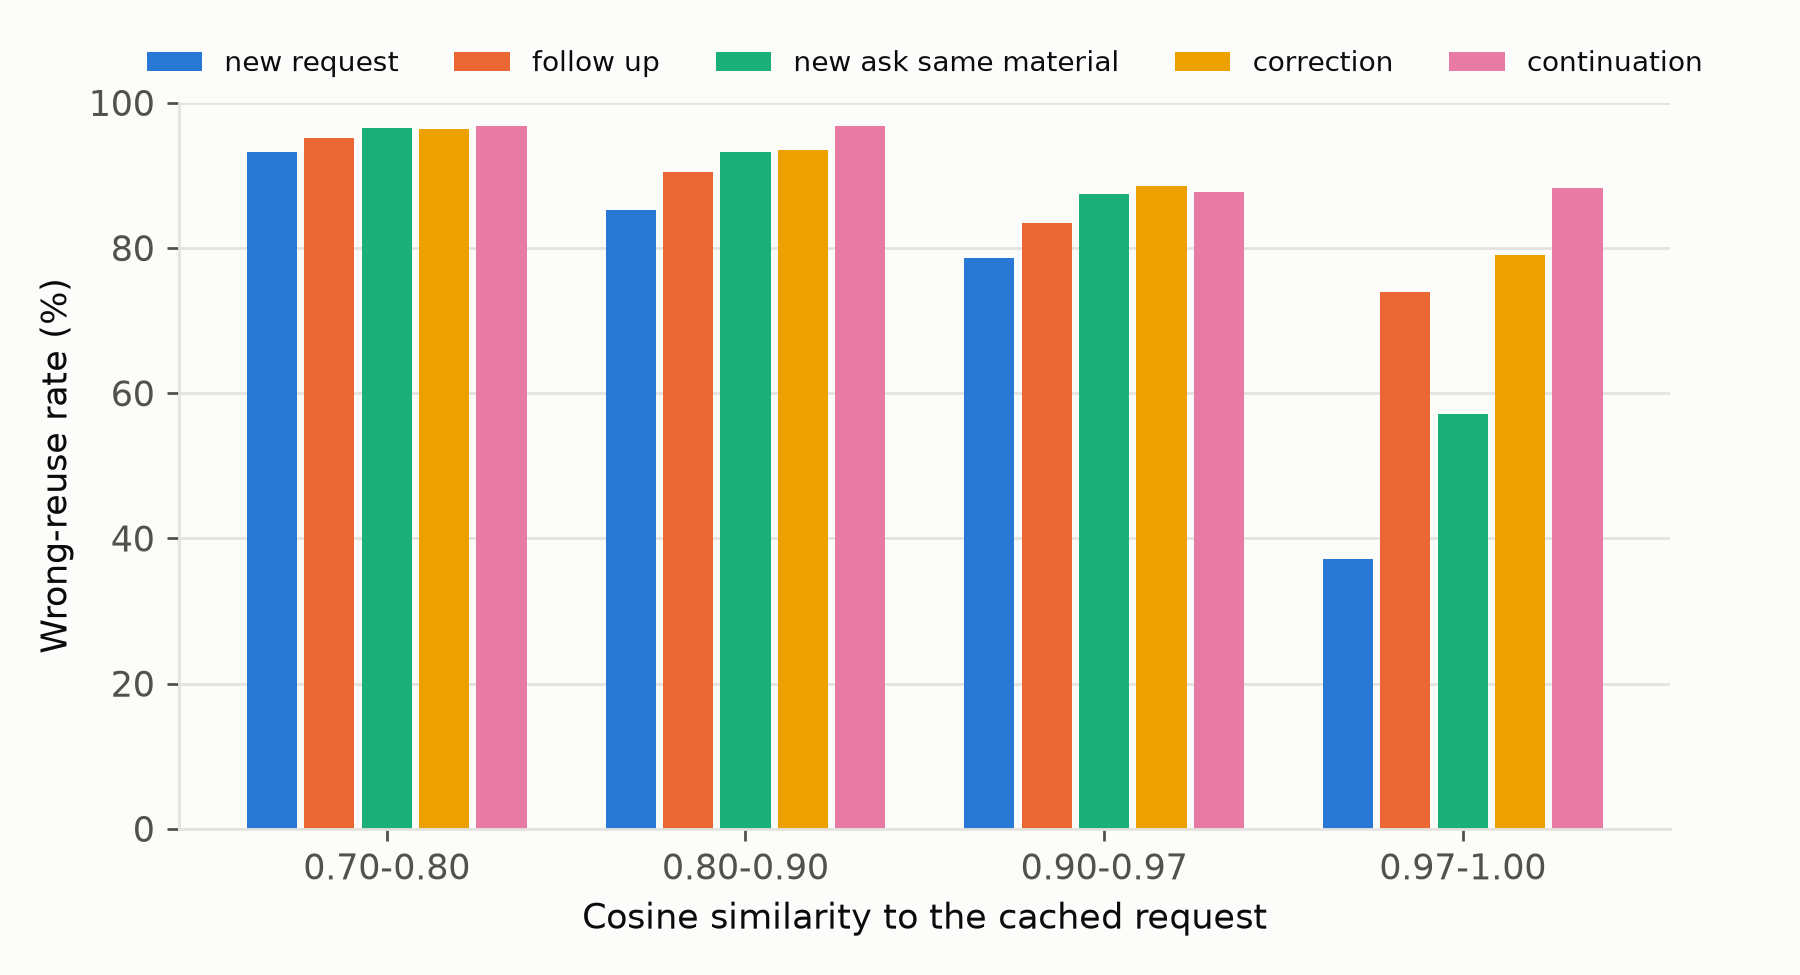
\includegraphics[width=\columnwidth]{figures/wrong_reuse_by_act.png}
\caption{Judged wrong-reuse rate by similarity band and dialogue act of the new request (all labeled pairs).}
\label{fig:finding}
\end{figure}

\begin{table*}[t]
\caption{Mined behavioral association rules with the lowest and highest reuse acceptability (training and development labels, at least 30 pairs)}
\label{tab:rules}
\centering
\footnotesize
\begin{tabular}{@{}llllrr@{}}
\toprule
Request state & Request act & Entry state & Entry act & Acceptable (\%) & Pairs \\
\midrule
start & new request & correction$\to$correction & correction & 0 & 34 \\
new request & follow up & new request$\to$follow up & follow up & 2 & 52 \\
new ask same material$\to$new ask same material & new ask same material & start & new request & 3 & 39 \\
follow up$\to$new request & follow up & new request & follow up & 3 & 30 \\
\midrule
start & new request & start & new request & 47 & 2643 \\
new request$\to$new request & new request & start & new request & 45 & 159 \\
start & new request & rare & new request & 44 & 43 \\
rare & new request & rare & new request & 39 & 108 \\
\bottomrule
\end{tabular}
\end{table*}

\subsection{Admission on the held-out period}
\begin{table}[t]
\caption{Confirmation period: hit rate (\% of all requests) at matched wrong-reuse with 95\% session-bootstrap intervals, and best net utility per 100 requests ($U=L=1$)}
\label{tab:main}
\centering
\footnotesize
\setlength{\tabcolsep}{3pt}
\begin{tabular}{@{}lccc@{}}
\toprule
Policy & HR@5\% & HR@10\% & Utility \\
\midrule
P1 fixed threshold & 0.02 [0.00, 0.17] & 0.02 [0.00, 0.26] & 0.95 \\
P2 per-intent thresholds & 0.80 [0.58, 1.07] & 0.80 [0.60, 4.34] & 2.71 \\
P3 per-turn verifier & 1.46 [0.21, 3.63] & 4.62 [1.65, 5.95] & 4.23 \\
P5 + context embedding & 1.27 [0.39, 3.97] & 3.87 [0.99, 5.05] & 4.10 \\
\textbf{P4 + mined patterns} & 1.12 [0.19, 3.61] & 4.49 [0.88, 5.71] & 4.04 \\
P4+ context and patterns & 1.83 [0.13, 3.89] & 3.80 [1.95, 5.69] & 3.87 \\
\midrule
\multicolumn{4}{@{}l}{Paired gains in points; $^\ast$ significant after Holm correction} \\
P4 $-$ P1 & +1.10 [+0.17, +3.61]$^\ast$ & +4.47 [+0.82, +5.67]$^\ast$ & \\
P4 $-$ P2 & +0.32 [-0.62, +2.62] & +3.69 [-1.54, +4.58] & \\
P4 $-$ P3 & -0.34 [-2.08, +0.92] & -0.13 [-2.21, +1.55] & \\
P4 $-$ P5 & -0.15 [-2.41, +1.22] & +0.62 [-1.68, +2.68] & \\
\bottomrule
\end{tabular}
\end{table}

\resultParagraph{}

\begin{figure}[t]
\centering
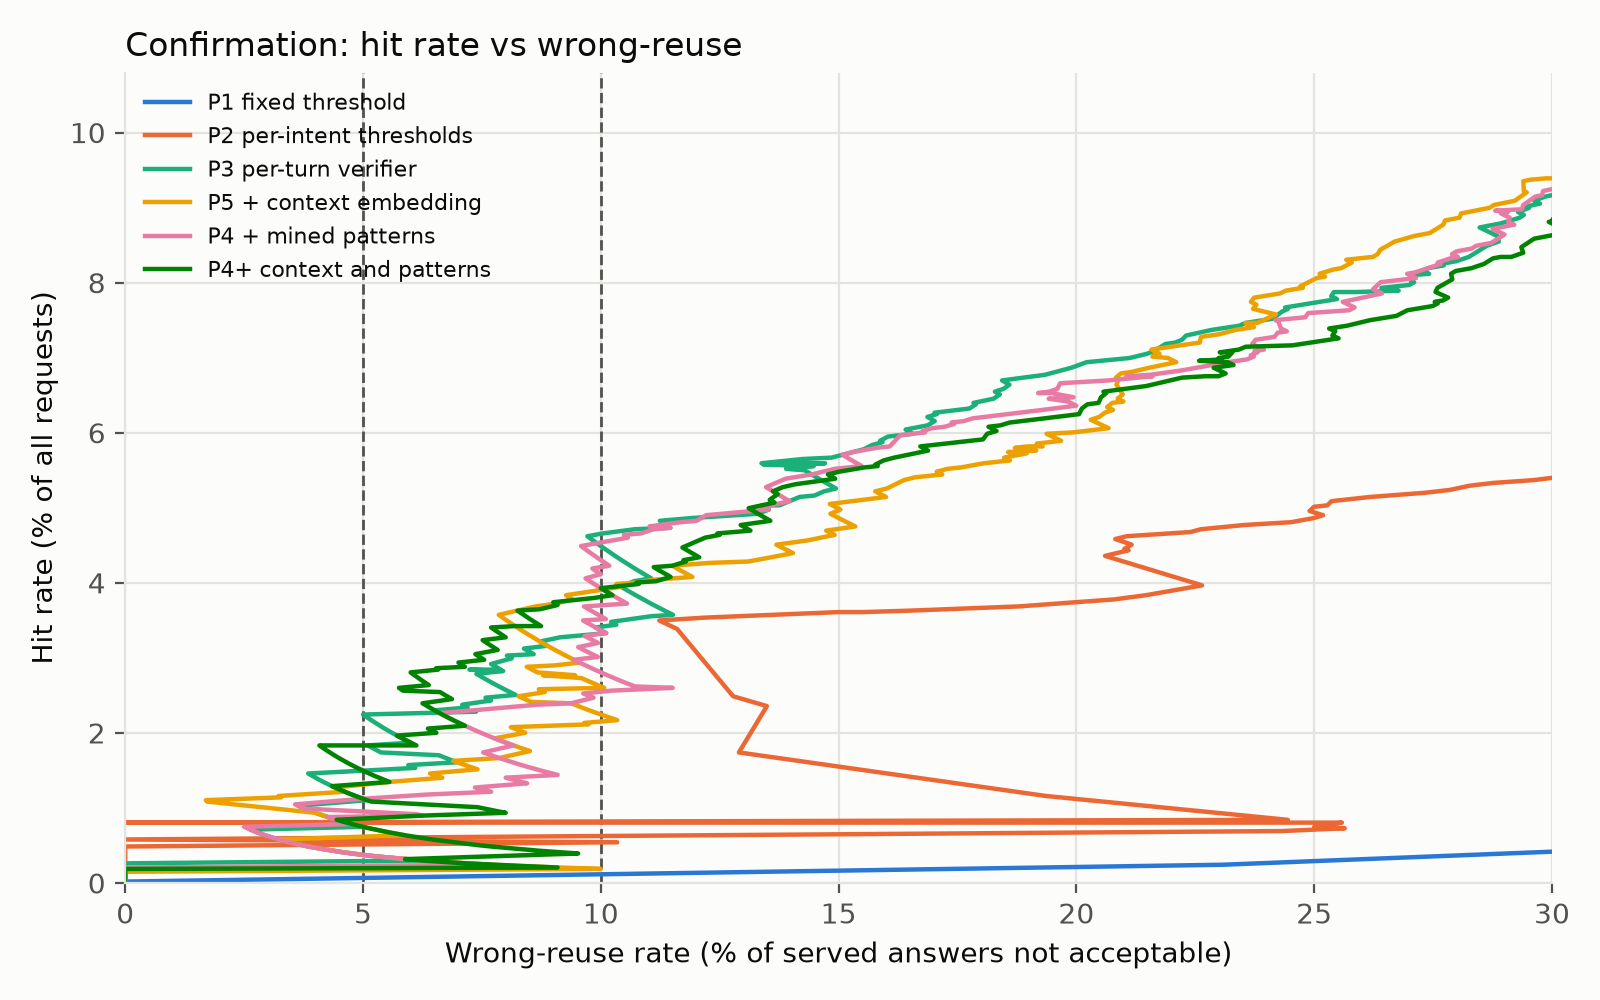
\includegraphics[width=\columnwidth]{figures/confirm_curves.png}
\caption{Hit rate against wrong-reuse rate on the confirmation period. Dashed lines mark the pre-registered levels.}
\label{fig:curves}
\end{figure}

\subsection{Controls, ablations and mechanism}
\begin{table}[t]
\caption{Placebos and ablations on the confirmation period (hit rate in \%; difference to P3 at 10\% in points)}
\label{tab:controls}
\centering
\footnotesize
\setlength{\tabcolsep}{3pt}
\begin{tabular}{@{}lccc@{}}
\toprule
Variant & HR@5\% & HR@10\% & $\Delta$ vs P3 @10\% \\
\midrule
P3 per-turn verifier & 1.46 & 4.62 & -- \\
Placebo: shuffled history & 1.27 & 3.87 & -0.75 [-2.42, +0.97] \\
Placebo: borrowed history & 0.84 & 4.71 & +0.09 [-1.44, +1.85] \\
Ablation: frequent only & 2.10 & 4.56 & -0.06 [-0.86, +1.68] \\
Ablation: sequential only & 1.35 & 4.77 & +0.15 [-0.71, +2.06] \\
Ablation: session only & 1.78 & 4.60 & -0.02 [-0.94, +1.67] \\
Ablation: user only & 1.16 & 3.85 & -0.77 [-1.50, +1.01] \\
Ablation: rule prior only & 0.86 & 4.21 & -0.41 [-1.63, +1.22] \\
Ablation: no rule prior & 1.81 & 4.42 & -0.21 [-1.24, +1.50] \\
\bottomrule
\end{tabular}
\end{table}

\controlsParagraph{}

\subsection{Routing}
\label{sec:routing}
\routingParagraph{}

\begin{figure}[t]
\centering
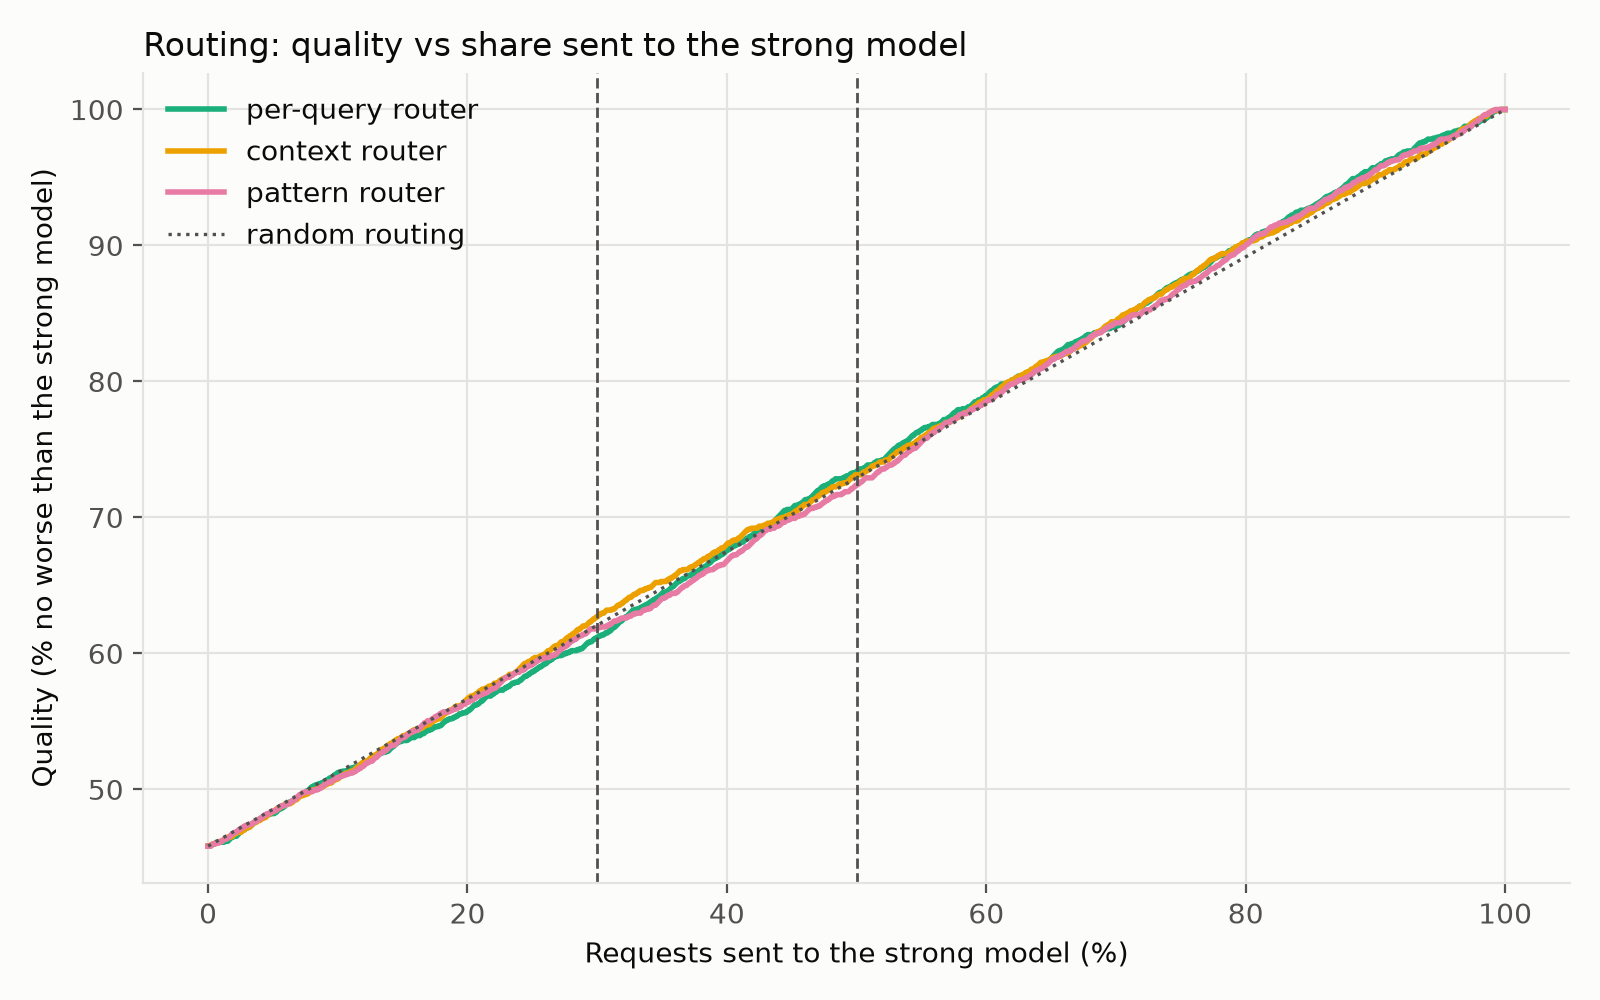
\includegraphics[width=\columnwidth]{figures/routing_curves.png}
\caption{Routing quality (share of conversations where the routed answer is no worse than the strong model's) against the share of requests sent to the strong model.}
\label{fig:routing}
\end{figure}

\subsection{Trajectory fast-tracking (exploratory)}
\label{sec:trajectory}
\trajectoryParagraph{}

\subsection{Deployment cost}
\serviceParagraph{}

\section{Threats to Validity}
The ground truth comes from an LLM judge; three models agreed on 85--88\% of pairs, and the human gold set provides the final check. Dialogue acts are LLM-tagged. The data are one public corpus over two weeks, and replay cannot capture how users would have reacted to a cached answer. The candidate pool is limited to the three most similar earlier turns per request. About 11\% of queued turns were not labeled; labeling followed a stratified random order and metrics are reweighted, so this reduces precision rather than introducing bias. Routing uses conversation-level human votes rather than turn-level outcomes.

\section{Conclusion}
Whether a cached LLM answer can be reused is, to a large degree, a behavioral question: the same words mean different things at the start of a conversation and in the middle of a refinement loop. Mining that behavior from gateway traffic, and turning it into association-rule priors over the states of both the request and the cache entry, gives an admission policy that knows when similarity is misleading. \conclusionSentence{} Future work includes live deployment in a gateway, turn-level routing outcomes, and trajectory caches validated with users.

\section*{Acknowledgment}
The authors thank Dr. Sandipan Maiti for guidance throughout this work.

\bibliographystyle{IEEEtran}
\bibliography{refs}

\end{document}
